\newpage
\section{Описание протокола}

На рисунке \ref{img:key_hierarchy} представлена иерархия ключей в EAP-PSK.

\begin{figure}[h!]
\center{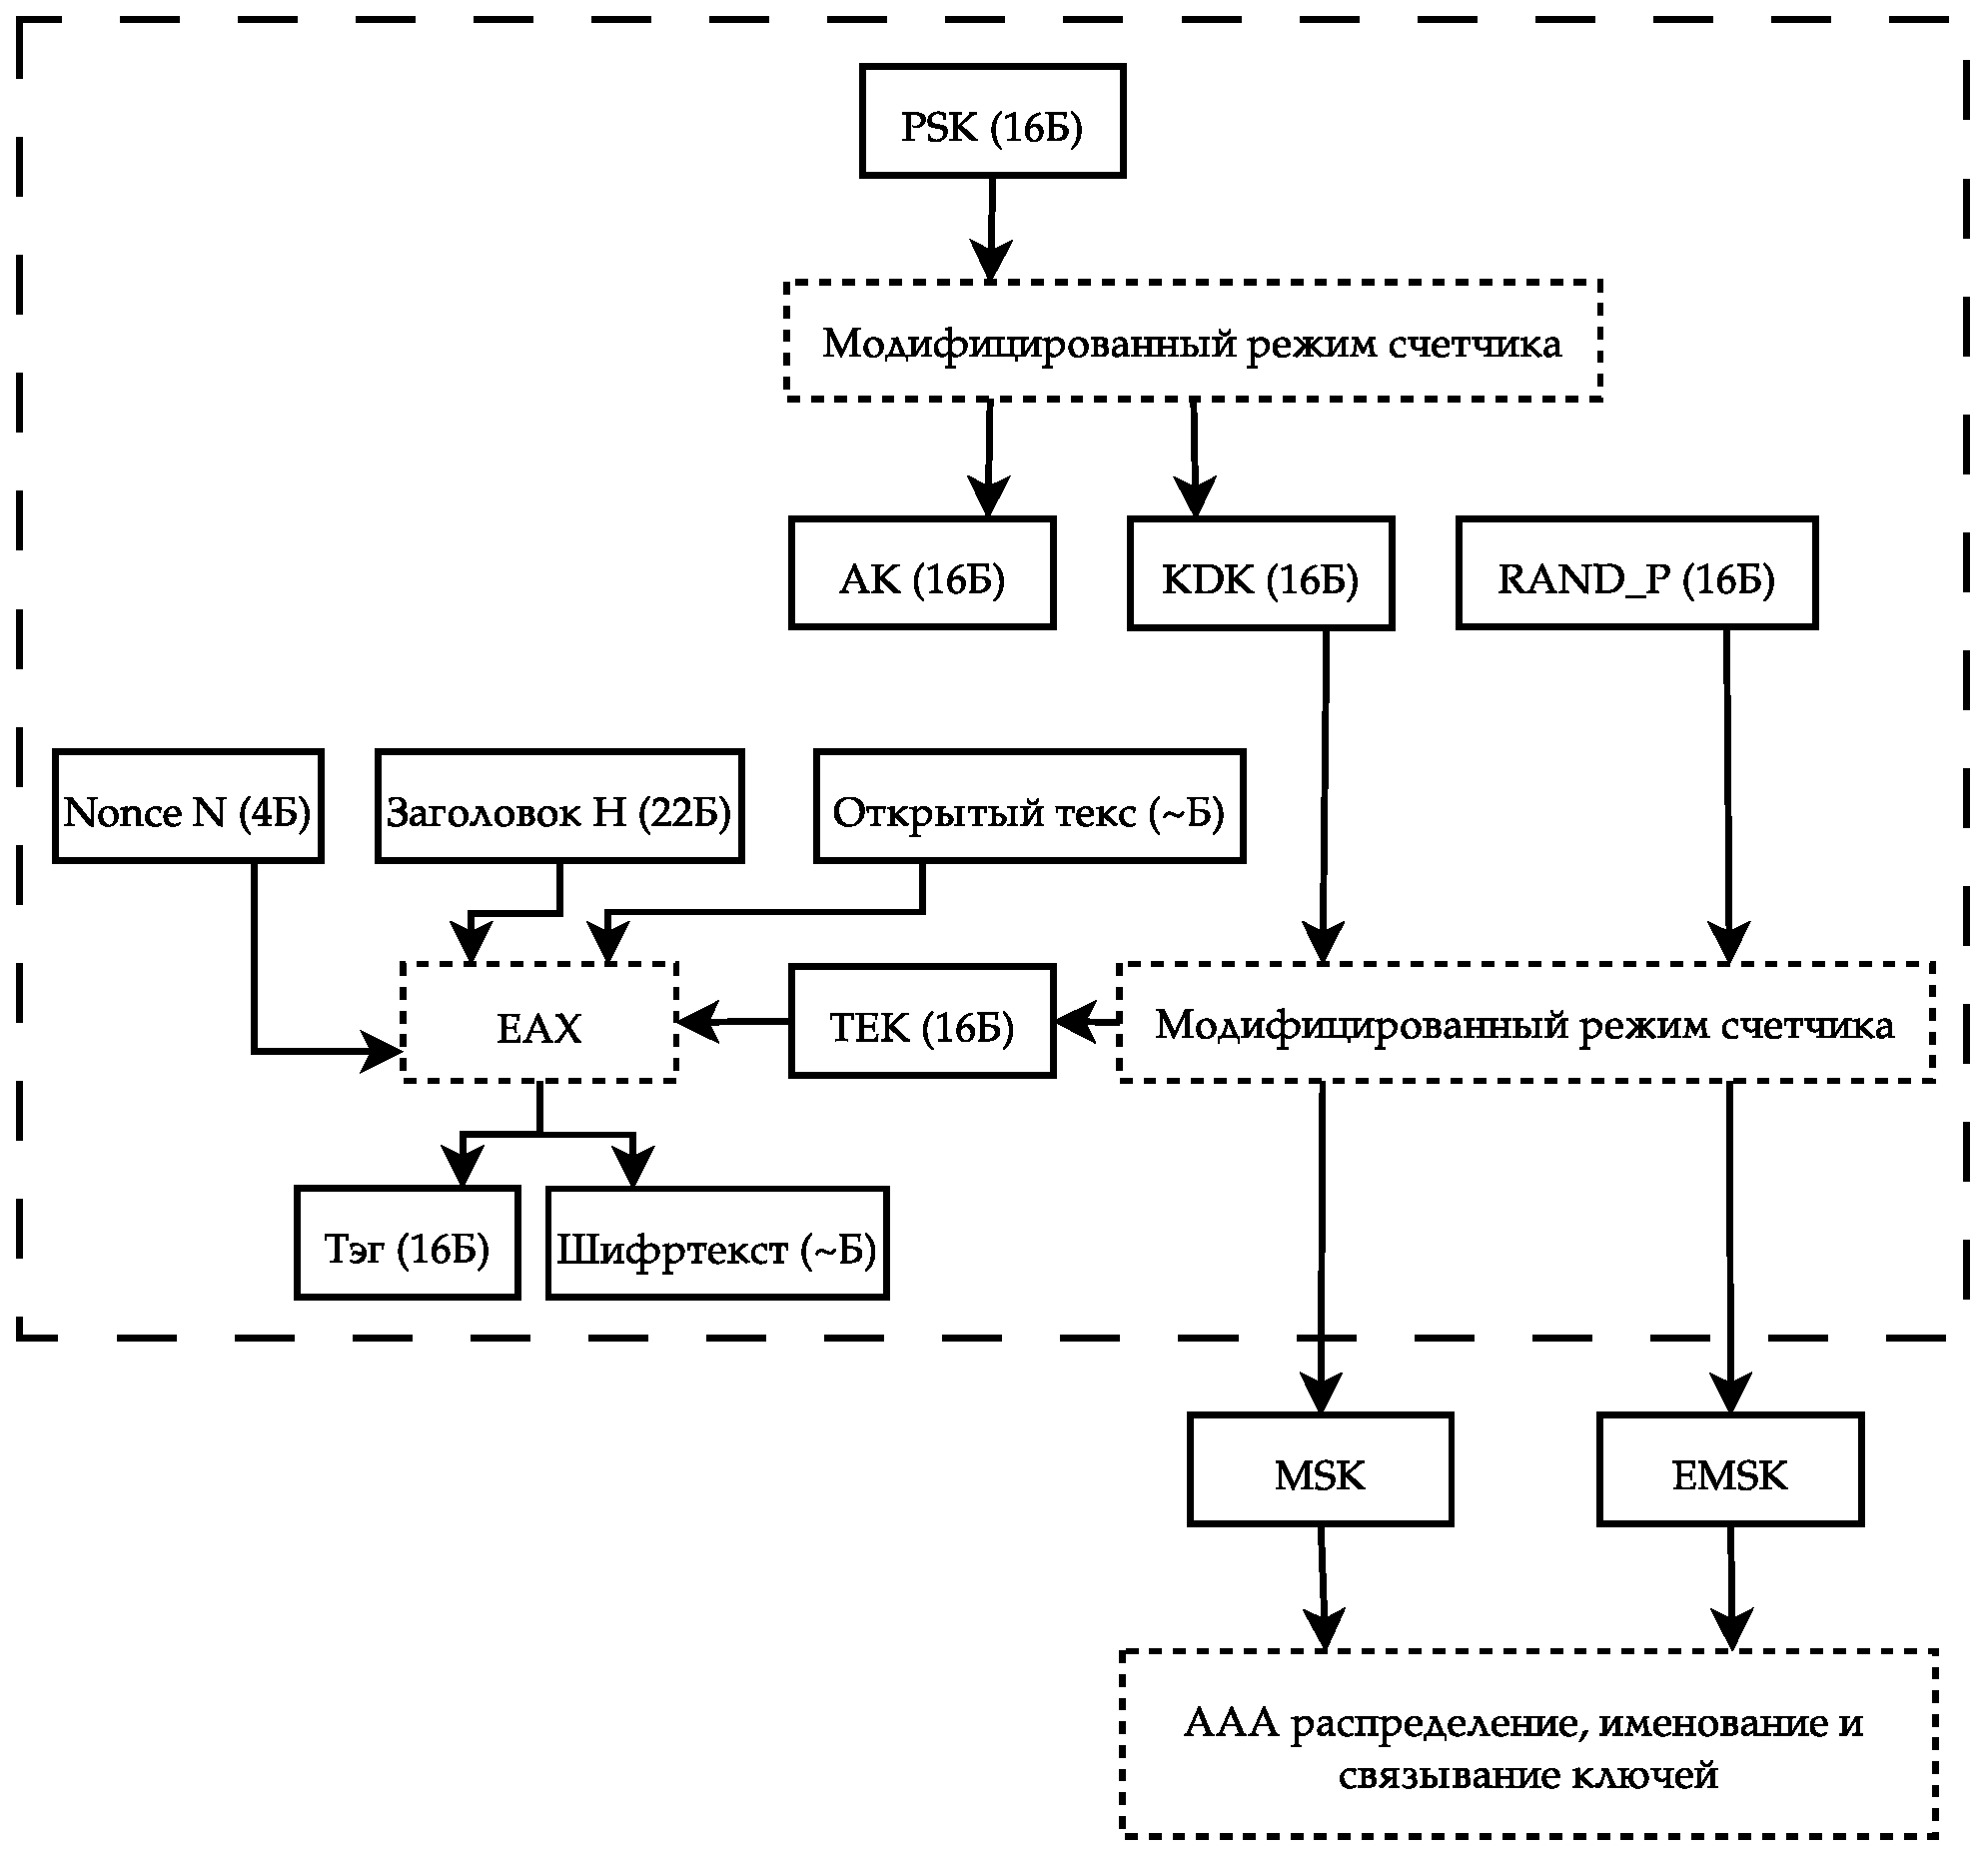
\includegraphics[width=0.9\linewidth]{./pictures/key_hierarchy}}
\caption{Описание иерархии ключей в EAP-PSK}
\label{img:key_hierarchy}
\end{figure}

\subsection{Иерархия ключей EAP-PSK}

В данном разделе описывается иерархия ключей, использующаяся в EAP-PSK. Эта иерархия базирутся на иерархии, оаисанной в документе ``Extensible Authentication Protocol (EAP) Key Management Framework''

\subsubsection{ПРедварительно заданный ключ PSK}

PSK распределяется между Пиром и сервером.

EAP-PSK предполагает, что PSK известен только Пиру и серверу. Распространение ключа другим обектам ставит под угрозу безопасность работы протокола. Это присуще не только EAP-PSK, но и всем протокола, использующим симметричные методы шифрования (включая так же парольные методы).

Так же предполагается что Пир и сервер устанавливают корректность используемого ключа благодаря их идентификаторам (NAI). Это означает, что у Пира и сервера с сответствующими идентификаторами может быть только один ключ.

Как показано на рисунке \ref{img:ak_kdk_psk}, PSK используется для генерации двух 16-байтовых долгосрочных ключей, называемых ключем аутентификации (AK) и ключем генерации ключей (KDK). Эти ключи должны быть сгенерированы единажды на этапе установки ключей. В разделе 3.1 данного документа объясняется почему PSK не используется как долговременный ключ, а используется только для генерации ключевого материала, используещегося EAP-PSK.

\begin{figure}[h!]
\center{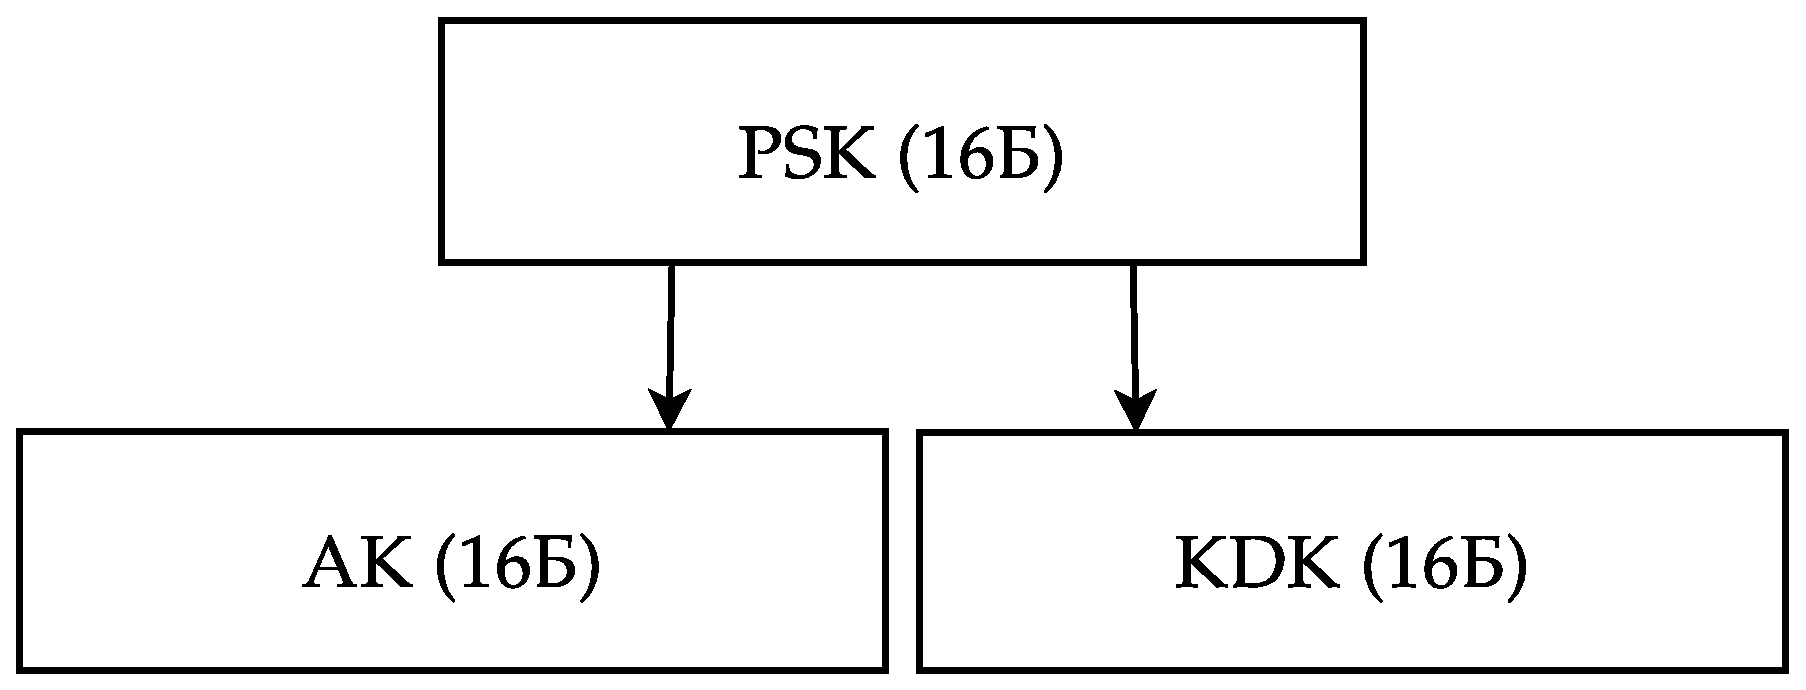
\includegraphics[width=0.9\linewidth]{./pictures/ak_kdk_psk}}
\caption{Генерация AK и KDK из PSK}
\label{img:ak_kdk_psk}
\end{figure}

\subsubsection{Ключ авторизации (AK)}

EAP-PSK использует ключ авторизации (AK) для взаимной аутентификации Пира и сервера. 

AK является долгосрочным ключем который генерируется с использованием PSK (см. раздел 3.1). Ключ авторизации не используется как сессионный ключ.

Пир и сервер выбирают необходимый AK для взаимодействия друг с другом основываясь на их идентификаторах (NAI). Это означает, что у Пира и сервера с сответствующими идентификаторами может быть только один ключ аутентификации. То же самое справедливо и для PSK (см. раздел 2.1.1).

Пир выбирает AK опираясь на NAI сервера, который был получен от сервера в первом EAP-PSK сообщении (а именно ID\_S. Раздел 4.1). NAI Пира включается во второе сообщение EAP-PSK (а именно ID\_P. Раздел 4.1).

\subsubsection{Ключ для генерации ключей (KDK)}

Ключ для генерации ключей (KDK) используется в EAP-PSK для получения сессионных ключей (а именно TEK, MSK, EMSK).

KDK является долгосрочным ключем и получается из PSK (см. раздел 3.1). Сам KDK не является сессионным ключем.

\subsection{Переходный EAP ключ (TEK)}

16-байтовый переходный EAP ключ вырабатывается во время процесса аутентификации путем обмена случайными числами (RAND\_P см. пункт 5.1); так же для генерации используется KDK.

TEK используется для установления защищенного конала обмена данными по которому будет происходить обмен данными для взаимной аутентификации.

\subsection{Мастер ключ сессии (MSK)}

MSK вырабатывается во время процесса аутентификации путем обмена случайными числами (RAND\_P см. пункт 5.1); так же для генерации используется KDK.

MSK, в соответствии с RFC3748, имеет длину в 64 байта.

\subsection{Расширяемы мастер ключ сессии (EMSK)}

EMSK вырабатывается во время процесса аутентификации путем обмена случайными числами (RAND\_P см. пункт 5.1); так же для генерации используется KDK.

EMSK, в соответствии с RFC3748, имеет длину в 64 байта.

\subsection{Вектор инициализации (IV)}

В соответствии с ``Extensible Authentication Protocol (EAP) Key Management Framework'' EAP-PSK не использует вектор инициализации.
